\chapter{Results}
\label{cha:results}

In this chapter, the micro-location method proposed in this paper---mediation---will be discussed in greater detail. A sample implementation of it is also provided along the paper. The whole method was implemented only in the Scala\footnote{\url{https://web.archive.org/web/20150817031402/http://scala-lang.org/} (visited on 08/17/2015).} language from the beginning to the very end. Scala is a compiled language and it compiles to JVM bytecode format, one that is widely used for server-side solutions, as well as for programming Android devices. Therefore, this choice allows for running the whole code completely off-line, in an Android application, or---equally easily---creating a web API accessible from any device. Functional--objective paradigm of the language (much like this of OCaml) allows for very concise and expressive notation of the ideas, as seen in some of the code listings in the following sections.

\section{Architecture of the proposed solution}
\label{sec:architecture}

\Cref{fig:architecture} presents the overview of main components of the solution. The process happens in several steps, some of which are repeated at each run, some need to be done once only.

\begin{enumerate}
	\item First, the data about locations used for micro-location purposes, that is held in human heads, needs to be digitized into computer-readable maps in OpenGIS format.
	\item At approximately the same time, configuration file for the micro-located object/place has to be created. In it, there are changes of costs defined that add or subtract from the total cost of a generated question, based on various properties and types of objects included in the question.
	\item The data contained in the maps is automatically transformed (parsed) into a format understood by the mediation engine\ldots
	
	\begin{figure}
		\centering
		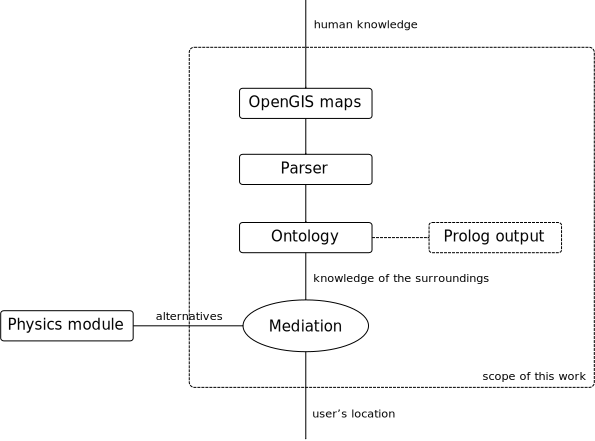
\includegraphics[width=\textwidth]{architecture}
		\caption{Architecture of the proposed solution (own work).}
		\label{fig:architecture}
	\end{figure}
	
	\item \ldots{}namely the ontology.
	\item An optional step that can be taken, is to export the ontology as a Prolog source code, that can be later used in some further research, as Prolog is particularly excelling at Artificial Intelligence prototyping.
	\item An external physics-based module needs to provide the mediation module with some alternative pre-guessed locations for the latter to choose from.
	\item Immediately after the alternatives are provided, the mediation starts. Using the knowledge of the surroundings (from the ontology) and rules concerning costs (from the configuration), several questions are presented to the user. Answers enable successful inference of their location.
\end{enumerate}

\section{OpenGIS maps}

Because of the fact that for all examples evaluated in this work (\cref{cha:evaluation}), parsing of their corresponding maps took less than a second, the parsing step is performed at each start time of the mediation engine. Thanks to that, the data is kept in its rawest form possible, i.e. just the maps. That makes it also easier for the administrative user, as no manual intermediate preparatory step is needed, when creating the data.

OpenGIS maps created for the sake of examples/evaluation in this work were made using the OpenJUMP\footnote{\url{https://web.archive.org/web/20150804110932/http://www.openjump.org/} (visited on 08/04/2015).} editor. This program creates a structure of files and directories corresponding to \emph{layers} defined by the user. A layer consists of several objects added to it at precisely defined position. The concept of layers doesn't play any role in mediation and thus they are only added as a convenience for the user creating the maps. Any object added to a layer---apart from its position in space---is also characterized by a map of properties in form of key--value pairs. In \cref{fig:opengis-props-map} such properties can be seen in the editor, while \cref{lst:opengis-props-onto} has these properties translated into Prolog source code. The properties are what has the greatest significance in the mediation process, as they enable discerning of objects; one of the properties takes a role of defining a class of an object (in ontological sense) and can be chosen at each parsing step.

\begin{figure}
	\centering
	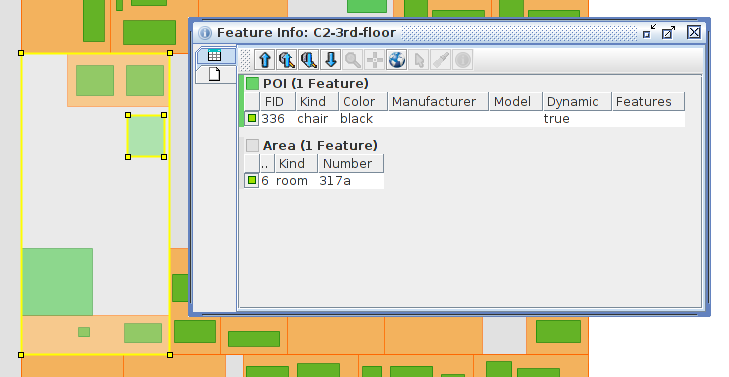
\includegraphics[width=\textwidth]{opengis-props-map}
	\caption{Properties of a ``chair'' object in OpenJUMP map editor.}
	\label{fig:opengis-props-map}
\end{figure}

\begin{lstlisting}[language=Prolog,caption={Ontology exported to Prolog source code for room ``317a'' containing the ``chair'' from \cref{fig:opengis-props-map} at line 10.},label=lst:opengis-props-onto]
room{number: "317a"} has [
  fridge{color: "white"} exists,
  desk{color: "light brown"} has [1
    microwave{color: "gray"} exists,
    kettle{color: "white"} exists
  ],
  wardrobe{color: "light brown"} has [
    display{color: "gray"} exists * 2
  ],
  chair{color: "black", dynamic: "true"} exists,
  wall{color: "white"} has [
    door{} exists * 2
  ]
].
\end{lstlisting}

\section{Ontology}
\label{sec:ontology}

At the beginning of the parsing process, all layers defined by the user are read into the memory. Each object on a map encountered during this phase is added to one big set of all objects. Such an object is characterized by its layer of origin, name of its class (e.g. ``door'', ``desk'', ``computer''), its geometry (where on the map it lies), and remaining properties (after using one for the class name), cf. \cref{lst:JmlObject}.

As seen in \cref{lst:opengis-props-onto}, optional export of the ontology to a Prolog format is supported, e.g. for further research. Also, dumping it like that makes debugging significantly easier, as the ontology that is used directly for mediation has no textual representation (e.g. frequent mentions in this section will call for the format to explain the ontology better).

\begin{lstlisting}[language=scala,caption={Definition of an object read from an OpenGIS map.},label=lst:JmlObject]
final case class JmlObject(origin: File, className: String, geometry: Geometry, props: Map[String, String])
\end{lstlisting}

Only after all objects are read, the geographical hierarchy begins to be established. An object is said to be an ``ancestor'' of another object, when geometry of the first covers geometry of the latter (i.e. the latter is geometrically contained in the first). This ancestry relation is obviously transitive. A ``parent'' of a ``child'' is this ``child'''s ``ancestor,'' where no other object can be found between the two. This particular relation is represented with the \texttt{has} keyword in the optional Prolog output (see \cref{lst:opengis-props-onto} for an example) and with a tree structure (see \cref{lst:JmlTree}) in the ontology used directly by the mediation engine.

\begin{lstlisting}[language=scala,caption={Definition of a (sub-)tree establishing the geometrical hierarchy and relations of OpenGIS objects.},label=lst:JmlTree]
final case class JmlTree(node: JmlObject, children: Set[JmlTree])
\end{lstlisting}

Because on the maps, there may---and probably will---be several disjoint top-level objects (e.g. rooms)---i.e. there does not necessarily have to be one big object to contain all the others---not only \emph{one} tree might have to be created, but a \emph{list} of such trees. To create the trees based on inclusions of geometries of the objects from the flat set, a modified form of topological sorting algorithm is used and the trees are built in a layer-by-layer fashion.

\begin{enumerate}
	\item First, objects with no ancestors at all have to be found.
	\item These objects are added to the next layer/level (``next'' being ``first'' in the first iteration) in appropriate subtrees in the list. Appropriateness is determined by ancestry (relative to the objects in a previous layer/level).
	\item These objects are also removed from the set.
	\item We go back to 1. until there are no objects left in the set.
\end{enumerate}

Initial plan for this project envisioned introducing other relations than just inclusion (the \texttt{has}). Later, these relations could be used in generating questions, enriching the pool of types of questions that the system can ask. However, the few sensible relations that the author was able to come up with and other significant drawbacks (discussed below) of such introduction, caused the decision not to include them.

\begin{description}
	\item[X exists] present in the ontology.
	\item[X has (consists of) Y] present in the ontology.
	\item[X is near Y] is symmetric, sometimes transitive (hard to tell when), needs context (hard to define), as nearness might mean completely different things depending on the room size (what if there is no room?).
	\item[X to the left/right of Y] is sometimes transitive, asymmetric, implicates ``is near,'' distributes over ``consists of,'' demands that both X and Y stay right next to the wall, needs context (analogically to ``is near'').
	\item[X is under/over/on Y] a slightly more detailed case of ``consists of'' that is not inferable just from the maps. (That one actually makes sense in generating a bit more naturally sounding questions: ``a computer on a desk'' vs. ``a desk with a computer.'')
\end{description}

Ambiguity of the relations above would cause the need to calculate them separately for every pair of objects, resulting in combinatorial explosion.

Another possibility for a question would be to ask for amount of things of certain type. That, however, would be highly inconvenient for the user (e.g. ``Do you see 7 or 9 computers?'' is much more difficult, demanding, time-consuming to answer than ``Do you see a black computer?'').

On the other hand, concentrating on ``exists'' and ``consists of'' is only lacking in an improbable situation of having two \emph{exactly identical rooms} regarding contents, but in which the contents are arranged differently. If one room contains at least one object that the other does not, they are perfectly distinguishable using just ``exists'' and ``consists of.''

\section{Configuration}
\label{sec:configuration}

In order to define costs of asking about different objects and properties of these objects, each location, apart from maps, needs to have a configuration file created. This file is parsed along with the maps, at each starting of the mediation engine. Costs are taken into account when choosing the best question to ask (more about that in \cref{sec:mediation}).

Such a file consists of 0 or more lines in the format of: \texttt{cost \underline{selector} $\pm$\underline{change}}. The \texttt{\underline{selector}} part is using lower-case property names and values as defined in OpenGIS maps (e.g. as in \cref{fig:opengis-props-map}). See \cref{lst:configuration} for an example of such file.

\begin{lstlisting}[caption={Definition of costs in a sample configuration file.},label=lst:configuration]
# a comment starts with a `#'
cost [] +50
cost [].color +10
cost [kind=computer] -15
cost [kind=mouse, color=black].model  +110
cost [kind=desk].[kind=mouse, color=black].model +10
\end{lstlisting}

Second line of \cref{lst:configuration} increases the default cost of asking about anything by 50 (e.g. ``Do you see a projector?'' would cost 50). In line 3, mentioning color in a questions, increases its cost by 10 (``Do you see a red projector?'' would cost $50+10=60$). Because spotting a computer is fairly easy, line 4 makes that explicit by decreasing a question mentioning computers by 15. Because of the definition in line 5, asking about a model of a black mouse is 110 more costly than the default. Costs definitions can also include information about ancestry (not only \emph{direct} parents, but grandparents, great-grandparents etc.), e.g. line 6 means that asking about a model of a black mouse lying on a desk costs 10 more, resulting in total cost of $50+10+110+10=180$ (the first 10 comes from line 3). Notice that asking about a computer's color would have the cost of $50+10-15=45$.

Such ``accumulating'' definitions allow for more consistency and compactness in the model, as it is harder for the defining user to forget about some corner case.

\section{Physics-based module for providing alternative possible user locations}
\label{sec:physics-module}

To get a few alternative locations (an input to the mediation process, ``where the user might be''), an external physics-based module is used. The one used currently is the subject of work of Bobek and Grodzki among others, and more about it can be read in \cite{bobek2015indoor, Koeping2015indoor}. Therein, details of mathematical models used are presented.

The basic idea is to use two sources of data. If inferred locations occupy more than one room, mediation is triggered. The sources are:

\begin{itemize}
	\item dead-reckoning (pedometer) using data from various motion sensors of a device (accelerometer, gyroscope) and
	\item strength of signals received from iBeacon-compatible transmitters placed in rooms.
\end{itemize}

Dead-reckoning (also known as ``inertial measurements'') works by changing the model's idea of user's location, incrementally adding and subtracting small changes to it (steps in this case). Amounts of these changes are inferred based on data coming from motion sensors of a devices using a mathematical model. As Köping et al. state in \cite{Koeping2015indoor}, ``We model the indoor localization problem as a recursive density estimation problem, which can be estimated by employing the Bayesian framework, namely particle filters.''

The idea for using beacons in the module is to make an assessment about distances to nearby transmitters based on signal strength and RSSI (one case of the law of inverse squares, see \cref{eq:inverse-sq} and \cref{sec:existing-uloc}). Arguably, this could potentially be seen as somewhat of a misuse of the iBeacon technology. Manufacturers generally speak of \emph{three} recognizable levels of ``interaction'' with the beacon (based on signal strength): \begin{itemize}
 	\item receiver being in very close proximity to the transmitter,
 	\item receiver being in the same room,
 	\item no interaction at all.
 \end{itemize}
 
Matyasik et al. claim that the RSSI-to-distance-based approach works, however, \emph{only under laboratory conditions} \cite{Matyasik:iBeacon, Matyasik:iBeacon:slides}. As iBeacons use extremely low energy to transmit the signal, even a single person walking across the room while taking the measurement---or even someone playing with the smartphone during the measurement---can influence it so negatively, that any information inferred about the distance to the signal's source cannot be reliably trusted.

\section{The process of mediation}
\label{sec:mediation}

The shortcomings of iBeacons and dead-reckoning (\cref{sec:physics-module}) on their own encourage the use of some additional data source. In this work, mediation is proposed.

In the provided sample implementation, alternatives from the list of trees (cf. \cref{sec:ontology}) are selected by \todo{alternatives can be provided in attr=val form; we can ask with high granularity}a list of key--value pairs corresponding with property names and values of objects in OpenGIS maps; e.g. to select rooms 317 and 318 in \cref{sec:case-agh}, one would have to specify \texttt{number=317} and \texttt{number=318} as the two alternatives; to select all rooms, \texttt would suffice.

In the implementation, mediation takes part in two modules.

\begin{enumerate}
	\item A sample and small (28 lines of code) \texttt{Mediator} that currently uses command line to present questions to the user and get their answers. 
	\item The \texttt{QuestionGenerator} that is the heart of the whole process. Given a list of alternatives---a list of \texttt{JmlTree}s, cf. \cref{sec:ontology}---it generates the best question possible to discern the alternatives, taking costs, objects, properties etc. into account.
\end{enumerate}

There are several question types defined, a super-type of which can be found in \cref{lst:question}. Each question type has to implement a map/dictionary of answers, in which an answer points to a set of alternatives that satisfy this answer (line 3). Each question also comes with a numerical cost directly obtained from the configuration file (line 4), a textual representation to show to the user (line 5), and a function returning textual representations of each answer (e.g. to put on some buttons in a user interface) (line 6).

\begin{lstlisting}[language=Scala,caption={Definition of a question super-type.},label=lst:question]
sealed trait Question {
  type Answer
  val answers: Map[Answer, Set[JmlTree]]
  val cost: Double
  val asText: String
  def asText(a: Answer): String
  
  final def entropy: Double = ...
  final def overallCost: Double = cost * (1.0 + entropy)
}
\end{lstlisting}

This very generic model of a question is sufficient to encode any question generated with any method. After all, it contains all information needed to choose the least expensive question from a set of questions, present it (with answers) to the user, and narrow down the set of possible user locations (which initially contains all the alternatives received from the physics module).

It turns out, that from this representation, it is also possible to calculate the \emph{entropy} of each question. Entropy here is a measure of uncertainty in the dataset, i.e. the smaller the entropy of a question, the better it discerns locations. E.g. a ``yes/no'' question that points to 2 locations when answered with ``yes'' and 0 otherwise will have much \emph{higher} entropy than one with 1 location pointed to by ``yes'' and 1 by ``no''.

\Cref{eq:entropy} is a classical definition of entropy $H$ for a dataset $S$, used in building decision trees (among others) \cite{quinlan1986induction}. Here, $X$ is a set of different classes in $S$. Also, $p(x)$ is a ratio of number of elements in class $x \in X$ to number of elements in the set $S$.

\begin{equation}
  \label{eq:entropy}
  H(S)=-\sum_{x \in X} p(x) \log_2 p(x)
\end{equation}

In calculating entropy of a question, it is necessary to calculate entropies of each of its answers first. In \cref{eq:entropy}, $X$ would be a set of locations pointed to by a given answer. Because $\vert x \vert = 1$ always (an answer can point only \emph{once} to a given location), and $\vert S \vert$ is equal to the number of different locations pointed to by the answer, $p(x)=\frac{1}{\vert S \vert}$ for all $x$. Therefore, \cref{eq:entropy} simplifies to \cref{eq:my-entropy-tmp} and in turn \cref{eq:my-entropy}.

\begin{equation}
  \label{eq:my-entropy-tmp}
  H(S) = -\vert S \vert \cdot \frac{1}{\vert S \vert} \log_2 \frac{1}{\vert S \vert}
\end{equation}
\begin{equation}
  \label{eq:my-entropy}
  H(S) = -\log_2 \frac{1}{\vert S \vert}
\end{equation}

In \cite{quinlan1986induction}, Quinlan provides a formula for calculating \emph{information gain} $IG(A)$ of splitting the dataset $S$ on an attribute $A$, see \cref{eq:information-gain}. I.e. this is the measure of uncertainty reduction in $S$ after it is split on $A$.

\begin{equation}
  \label{eq:information-gain}
  IG(A,S) = H(S) - \sum_{t \in T} p(t)H(t)
\end{equation}

Here, $T$ represents all subsets created when splitting $S$ by $A$ such that $S = \bigcup_{t \in T} t$ and $p(t)$ is the ratio of the number of elements in $t$ to the number of elements in $S$. As $H(S)$ is always constant, it can be neglected when comparing questions. Entropy of the whole question is then defined as just $\sum_{t \in T} p(t)H(t)$. In this case, $t$ represents one answer of a question and $\vert t \vert$ is the number of locations pointed to by the answer. After some substitutions we arrive at \cref{eq:question-entropy}, a formula for the entropy of the whole question.

\begin{equation}
  \label{eq:question-entropy}
  \sum_{t \in T} \frac{\vert t \vert}{\vert S \vert}\left(-\log_2 \frac{1}{\vert t \vert}\right)
\end{equation}

Overall cost of a question has to combine both the entropy (\cref{eq:question-entropy}) and costs inferred from the configuration file \cref{sec:configuration}. The formula in line 9 of \cref{lst:question}, namely $overallCost = configurationCost \cdot (1 + entropy)$, has been found to be particularly useful.

See \cref{sec:case-agh} and \cref{sec:case-cracow-square} for sample mediation sessions. At each point during such a session, the mediation engine strives for complete intelligibility by showing the user how their answers affected which alternatives remained in the set of their possible locations.

It is worth noting, that Köping et al. in \cite{Koeping2015indoor} suggest a different method of generating questions.


\todo{Slażyński and Bobek propose alternative method but\ldots why ask 2+ questions when there are only 2 alternatives; either one suffices or they are indistinguishable; prolog impl cannot be run on Android}



\todo{finish}

\section{User Experience}
\label{sec:user-experience}

\todo{finish}
